\chapter{绪论}{Introduction}
\label{chap:intro}


XXX 开场白,主要介绍对话系统的blah blah,然后点出本文主题

      从人工智能发展的早期开始,人们已认识到人机通过自然语言交互在机器智能领域的关键性作用。在1950年,Alan Turing发表了他的那篇经典文章“计算机与智能化(Computing  Machinery and Intelligence)”。在文章中,他提出了一个如何判定机器是否智能的标准,现在称其为“图灵测试”。他并没有称这个标准为“智能对话系统”,但对于任何系统来说,要通过图灵测试,能实现人与机器通过自然语言进行交互的智能系统显然是至关重要的。

%%%%%%%%%%%%%%%%%%%%%%%%%%%%%%%%%%%%%%%%%%%%%%%%%%%%%%%%%%%%%%%
\section{研究目的和意义}{Background}
%%%%%%%%%%%%%%%%%%%%%%%%%%%%%%%%%%%%%%%%%%%%%%%%%%%%%%%%%%%%%%%
XXXX

%%%%%%%%%%%%%%%%%%%%%%%%%%%%%%%%%%%%%%%%%%%%%%%%%%%%%%%%%%%%%%%
\section{研究现状综述}{The State of the Arts}
\label{sec:review}
%%%%%%%%%%%%%%%%%%%%%%%%%%%%%%%%%%%%%%%%%%%%%%%%%%%%%%%%%%%%%%%

对话系统简单来说就是计算机用来试图和人类通过自然语言交流的软件系统。对话系统的思想可以追溯到1950年图灵在\cite{Turing1950}中提出的图灵测试,在过去的几十年中,有关对话系统的研究大致有两个不同的方向:一个是仅在表面外观上模拟对话,也被称为聊天机器人,如著名的聊天机器人心理医生ELIZA\cite{Weizenbaum1966}等。这类系统大多数不考虑理解对话内容的含义,直接采用模板匹配的方式找到和用户输入相关的对话,目前经常被用在各类社交网站和实时通讯的社交软件中。另一个是试图模拟人类真实的对话,并动态产生合适的对话,也被称为对话管理。后者是本文的研究重点,因此这一小节我们将回顾这一类对话系统以及对话管理的相关研究。

目前,对话系统的研究中有很多不同的架构体系,一个对话系统包含哪些功能模块也视不同的系统而异,但一般来说,对话系统主要包括以下几个功能模块:自然语言理解模块、对话管理模块、知识表示模块、自然语言生成模块\cite{Arora2013}。各模块之间的数据走向如图\ref{fig:dialogue}所示。接下来我们将分别就对话系统中的各个功能模块来展开综述相关研究现状。另外,由于本文的智能对话系统中使用了言语行为理论的启发和指导,因此也会在本节对其相关研究进行简明的阐述。需要说明的是,本文研究的对话系统暂时只是基于文本的,所以这里暂且不讨论语音识别和语音合成模块。

\begin{figure}[htb]
\centering
\includegraphics[width=12cm]{figures/dialogue_system.png}
\caption{对话系统的基本结构}
\label{fig:dialogue}
\end{figure}


%%%%%%%%%%%%%%%%%%%%%%%%%%%%%%%%%%%%%%%%%%%%%%%%%%%%%%%%%%%%%%%
\subsection{知识表示及相关逻辑推理研究综述}{Overview of Knowledge Representation And Logic Reasoning}
\label{sec:representationReview}
%%%%%%%%%%%%%%%%%%%%%%%%%%%%%%%%%%%%%%%%%%%%%%%%%%%%%%%%%%%%%%%

对于任何以实现复杂功能为目标的自然语言处理系统(如对话系统或复杂的问答系统)来说,该系统内部的知识表示形式,即如何表示语义处理后的自然语言,往往是系统的各方面性能表现的关键所在。本小节将介绍知识表示目前的研究现状并回顾一些典型的知识表示方法及相应的优缺点,我们也会在本节重点介绍与本文所采用的知识表示相关联的几个具有代表性的知识库。

如何合理有效地表示自然语言话语的含义是过去50年来一直被争议的问题,这也是从一个句子中抽取信息的语义建模问题所面临的第一步。然而目前,“知识表示”需要满足哪些条件仍然处于争论状态。Jurasky和Martin在经典的《自然语言处理综论》\cite{Jurafsky2009}的第14章中从不同方面总结了一个完整的知识表示体系所要满足的计算需求,其中包括:

\begin{itemize}
\item 可能性验证(Verificability):必须能够确定知识表示的真实性,即知识表示体系能将输入的命题表示与储存相关知识的世界知识库中的表示相比较或匹配。
\item 无歧义表示(Unambiguous Representation):知识表示的语言支持的表示只能有一个无歧义的解释。
\item 规范形式(Canonical Form):表达同样信息的输入必须具有同样的知识表示形式,即规范形式。
\item 推论与变元(Inference and Variables):知识表示体系能根据输入的知识表示以及储存的背景知识推理出可靠结论。
\item 表达能力(Expressiveness):知识表示方法需要具备足够的表达能力来处理各种广泛领域的知识。
\end{itemize}

直到最近,这些需求列表一直被当做是知识表示领域中一个相当完善的黄金标准。Yarin等人\cite{Yarin2013}指出了这个必要条件列表并不完整,并指出了知识表示体系还需满足下列需求:

\begin{itemize}
\item 不确定性和内涵的表示
\item 能使用可行的方式来抽取话语的信息(即,从数据中抽取相关知识表示的算法的需求)  
\item 从话语中推理出相对应的情感和观点
\item 从不同命题中获取相关的不确定性
\item 不仅需要区分具有不同的意义的话语,还需区分涉及相似意义的话语
\item 在从话语中获取活动信息的同时还要获取活动相关的动作者(agent)
\item 回答问题除了使用相关的知识外,还需要能利用这些知识和问题的意义。
\item 对同一个意义,能生成不同表达方式的话语
\end{itemize}

当然这些需求本身也没有得到相关的验证是否就完全,但近几年提出的一些知识表示方法及相关研究也在试图满足这其中的部分或所有需求。下面我们将简单回顾一些具有代表性的知识表示方法以及相应的优缺点,从中也不难看出未来知识表示领域的研究方向。知识表示的任务比较繁琐,所涉及的领域比较广,因此很难有一个完整的分类体系来概括所有的知识表示方法,本文通过以下几方面来分类介绍典型的具有实用价值的知识表示方法。

\begin{enumerate}
\item {传统的知识表示方法}

这里的传统的知识表示方法主要指逻辑表示法、框架表示法以及语义网络表示法,以及在这基础上的一些延伸表示方法,下面将对这几类典型的传统知识表示方法做简单的分析和对比。

\begin{enumerate}
\item[1)] 逻辑表示法

逻辑表示法的思路是将自然语言话语转换成某种逻辑约束下的一组逻辑表达式,以及在该逻辑上对这些逻辑表达式的语义解释。常见的用于知识表示的逻辑有命题逻辑,传统逻辑以及谓词逻辑等。对复杂的自然语言来说,命题逻辑和传统逻辑的表达能力相对弱,这里主要介绍基于谓词逻辑的知识表示方法。

谓词逻辑表示法中既包括一阶逻辑也包括高阶逻辑(如多个量词)的表示,但从实用角度来看,也就是在有限数量信息的下,两者之间可以通过一定的逻辑等价推理来转换,而一阶逻辑具有简洁和易推理的优点,因此相对来说更广泛地被应用,也是被研究地相对成熟的一种知识表示方法。

基于一阶逻辑的知识表示体系中使用了三种基本构件:常量(有时也称为原子atom),函数以及变量,每一个构件都指向世界知识中的某个对象。其中,常量通常用于表示世界知识中的对象,比如“狗”;函数通常定义在常量或者变量上,在自然语言的背景下,“函数”可用于产生新的词汇。比如函数“Black(狗)”可生成“黑色的狗”或者“黑狗”;变量则允许我们表达对非具体对象的陈述或预测。将这三个简单的构件和存在量词以及连接符号和否定关系符号,我们可得出以下的表达式用于表示“存在一个实体,这个实体拥有一只黑色的狗,并且给这只黑色的狗喂了红色的肉。”

$$ 
\exists X(Own(X, Black(Dog))\land Feed(X, Black(Dog), Red(Meat))) 
$$


在上述的逻辑表达式上,我们可以进行相关的逻辑推理和蕴含等操作,并且能通过\lambda表达式来确定命题的真值。一阶逻辑表示法允许我们将自然语言话语表示成一种无歧义的表示方式。对于多义词,我们可以采用多个常量(原子)来表达,比如可以用$Bank_{institution}$来表示意思为“银行”的"Bank",用$Bank_{institution}$来表示意思为“河岸”的"Bank"。此外,这种表示方法的表达能力也适用于表达多个句子的情况。

比较典型的使用一阶逻辑的知识表示体系有早期的Cyc系统\cite{Lenat1990}。Cyc系统拥有一个非常丰富的人工编码知识库,它的终极目标是:以谓词逻辑的形式,将所有人类常识进行编码。虽然它的知识库中已存有数百万的谓词逻辑表达式,但到目前为止,似乎只对一小部分人类常识进行了编码。

一阶逻辑的知识表示方法相对简洁,但由于自然语言的复杂性和不确定性,如何将自然语言话语转换成一阶逻辑的表示形式,是一个极大的挑战。Pianatadosi等人\cite{Piantadosi2008}首先在几十个词的限定条件下构建一个概率模型,使其能对各种可能的语法建模并过滤掉过于复杂的,从而根据这些语法模型来得到相应的一阶逻辑表示形式。在此基础上,他们的研究还深入到通过递归方式来遍历所有可能的上下文无关文法的概率模型,使得递归进行到一定程度能得到一个对话语进行最佳解析的一阶逻辑表示形式。该方法最终能得到一个不可扩展的在迷你规模语法基础上的组合语义获取模型,并没有实用价值。

后期的Cyc系统也为了克服一阶逻辑表示方法的缺点,引入了贝叶斯网络来为该知识库中的概念和事件提供相应的概率真值,但后期Cyc系统也转入商业用途,其数据和表示也不免费公开,因此我们尚不清楚目前其具体研究状况。

\item[2)] 基于框架的知识表示法

基于框架的知识表示方法又被称为槽填充表示法。框架(Frame)可以理解成一种将某一对象或事件所涉及的知识信息存储在一起的复杂的数据结构,通常包括主体和槽(Slot)两部分,其中主体是固定的,表示一个特定的概念、对象或事件,而槽用于表示主体的各属性及属性值。其一般形式可以表示如下:

       <主体>  

       <槽名1><槽值1>| <侧面名11><侧面值111,侧面值112,…>

                                    <侧面名12><侧面值121,侧面值122,…>

比如“我吃蛋炒饭”可以表示成框架形式如下:

       <吃>  

       <施事者><我>

       <受事者><蛋炒饭>


基于框架的知识表示常被用于语义角色标注中,即标注出句子中的谓词以及相应的参数。比如“我吃蛋炒饭”,语义角色标注可以标注出其中谓词是“吃”(框架主体,表示事件),该事件的槽值可以表示为施事者“我”,受事者“蛋炒饭”。

基于框架的表示法具有代表性的系统有FrameNet\cite{Atkins95}, FrameNet是一个人工编写的基于框架的语义知识库,其中包含了1,200个语义框架,13,000个词汇单元,大约19万个例句,目前被广泛用于语义角色标注的训练语料。

The process of capturing first order logic and frame based representations
from utterances is not trivial however.

基于框架的表示形式也可以很容易被转换成等价的一阶逻辑表示形式。与一阶逻辑表示相似,将自然语言话语转换成基于框架的表示形式也是该表示方法的巨大挑战。

\item[3)] DSC树\cite{Liang2013}
Liang, Jordan, and Klein (2013) have suggested reducing the task to a simpler
problem of constraint satisfaction, and by that allowed for efficient inference
to be carried out. They developed a new representation called DCS trees – dependency
based compositional semantics trees – and map utterances to these
trees in an efficient way through the constraints of pre-specified trigger words
and a predicate dictionary given in advance (for example the word city would
trigger the predicate city). Although the model was assessed on small scale
data-sets with some limitations for scalability originating from the specification
of trigger words, it can easily be scaled-up to map sentences over much larger
domains through the use of role-labelled input and shallow extraction of predicates
from text. Together with recently published large scale fact data-sets such
as Freebase (Bollacker, Evans, Paritosh, Sturge, and Taylor, 2008) this model
will allow for scalable question answering to be carried out extending on existing
question answering systems that rely on simple role-labelling and empty slot
completion based on previously observed statements.

However the developed representation, studied thoroughly in (Liang, 2011),
lacks a formal proof for the expressive power it offers. It is unknown yet whether
all sentences expressible in first order logic can be captured using DCS trees and
their possible extensions. Furthermore, the formulation of DCS is analogous to
and inspired by that of database querying languages (from personal communication
with Liang). But even for these well studied database querying languages
it has been shown that the expressiveness offered is very limited (Libkin, 2001).
It has been shown that small differences in the language definition affect the
behaviour of the language dramatically and that these languages cannot define
recursive queries regardless of the aggregate functions and arithmetic operations
specified (these recursive structures can, however, be observed in natural language).
Furthermore, it was shown that the problem of proving expressiveness
bounds for these is as hard of a problem as some long-standing open problems
in complexity theory (Libkin, 2001).

The use of a database querying languages for the representation of natural language utterances and not just knowledge by itself is a very interesting idea that allows for efficient logical inference and entailment to be carried out in the form of constraint satisfaction, and indeed has been studied before
(Giordani and Moschitti, 2010a; Monteleone, di Buono, and Marano, 2013;
Giordani and Moschitti, 2009, 2010b). However, even when justified with the
explicit assumption placed in advance of capturing only a subset of language
utterances, there is still the question of which representation to choose. The
mapping of utterances to the SQL query language offers the advantages of the
well studied language1
. The expressive power of DCS is still an open problem
to be explored.


\item[4)] 语义网络表示法:ConceptNet \cite{Robert2012}


ConceptNet's new reference, Representing General Relational Knowledge in ConceptNet 5\cite{Robert2012}

知识表示的另一个模式是由ConceptNet提供的\cite{Liu2004}。它从Cyc系统和形式逻辑中借鉴了一些理念,但没有考虑复杂的位元,如量词,并且比较接近自然语言层面。ConceptNet 是个大规模的语义网络,它表达概念(由单词或短语表述)之间的关系。图\ref{fig:concept}是关于子网络的例子。

\begin{figure}[htb]
\centering
\includegraphics[width=12cm]{figures/conceptnet.png}
\caption{ An illustrative fragment of ConceptNet }
\label{fig:concept}
\end{figure}

\end{enumerate}

All the representations above can be thought-of as rigid representations as
they do not capture uncertainty in the logical inference and entailment process.
For this reason \cite{Poon2009} have suggested a probabilistic representation
to do so. The representation used was chosen to be Markov logic \cite{Domingos2007}, a representation that allows one to capture
logical entailment as well as uncertainty. However, since the representation was
limited to its most basic form allowing no complex first order logic statements to
be captured, follow-up research by  \cite{Titov2011} has neglected
it in favour of a simple role-label representation, where hierarchical Pitman-Yor
processes were used to model statistical dependencies between predicates and
their arguments2. There are many other alternative representations suggested
for probabilistic logic; some of them will be discussed next.



Follow-up Research for "no complex FOL statements to be captured\cite{Titov2011}

\item {基于概率逻辑的知识表示法}

XXX这节需要用到的文献列表XXX

Probabilistic Representation \cite{Poon2009}

Markov Logic\cite{Domingos2007}

efficient logical inference \& entailment in the form of contraint satisfaction\cite{Giordani2010a},\cite{Giordani2010b}, \cite{Giordani2009}

PLP, BLP\cite{Kersting2007}

Probabilistic Similarity Logic\cite{Brocheler2012}

Probablistic Logic Representation has two contrasting interpretations\cite{DaRaett2003}




\begin{figure}[htb]
\centering
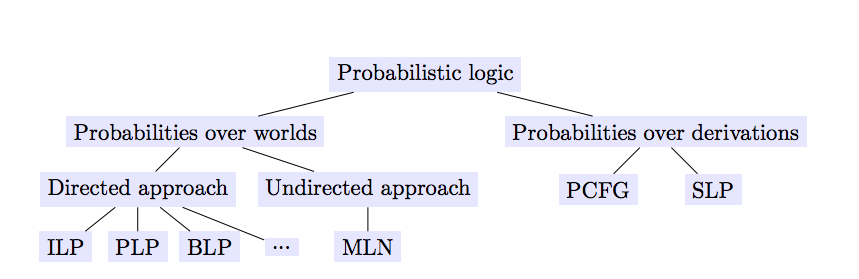
\includegraphics[width=12cm]{figures/plr-relation.png}
\caption{概率逻辑的不同表示形式的分类}
\label{fig:plr-relation}
\end{figure}

\begin{enumerate}

\item[1)] Probabilities over different worlds
XXXX

\item[2)] Probablities over derivations
XXXX

\item[3)] Probablities over experience: PLN, NARS
XXX语言需要调整XXX
Pei Wang的NARS引擎运用了传统逻辑推理法\cite{Wang2006},并引入了独特的数学运算,用于管理与“传统逻辑关系”有关的不确定性。NARS是建构在经验的基础上,而不是模型论语义学。

在许多方面,我们所使用的PLN逻辑形式化体系与NARS有类似的地方,但也存在巨大差异。PLN在一个独特的数学框架下,同时利用传统逻辑和谓语逻辑。此外,PLN还使用概率数学,以推导不确定真值的公式。反之,NARS是基于原始的、非概率的、不确定的管理体系。PLN也是以经验语义为基础,但形式与NARS不同。


图\ref{fig:nars}展示了基本演绎推理、归纳推理和外展推理公式。这些公式是PLN和NARS共有的。在每个关系式右边的$<s,c>$表示“每个关系的强度和置信度”。PLN和NARS使用不同的公式,从那些前提中推导(优势、信息)结论的真值。

\begin{figure}[htb]
\centering
\includegraphics[width=12cm]{figures/nars.png}
\caption{ NARS/PLN 传统逻辑中演绎推理、归纳推理和回溯推理的形式 }
\label{fig:nars}
\end{figure}


\end{enumerate}

\item  {分布式知识表示法}



\item  {Compositional Distributional Representation}

XXX这节需要用到的参考文献

Nouns as vectors, Adjectives as matrices linearly transforming these nouns\cite{Baroni2010}

For Compistional Distributional Representation, the use of linear projections can be identified with non-quantified FOL\cite{Grefenstette2013}

\end{enumerate}






目前的知识表示体系都在一定程度上为了简化推理过程而牺牲其表达能力。


XXX下面部分语言要稍微调整一下XXX




Atomspace是开源的认知体系结构OpenCog\footnote{\url{http://wiki.opencog.org/w/The_Open_Cognition_Project}}里所使用的知识表示体系,也是本文所采用的知识表示机制,会在第\ref{chap:representation}中进一步介绍,这里只对比它和目前存在的一些知识表示方法的比较。

Atomspace与ConceptNet有些共同之处。我们视Atomspace为“加权标记超图”,但ConceptNet只是一个“加权标记图”。此外,在可以直接表示的关系复杂性方面,Atomspace与ConceptNet有所不同。Atomspace包含与ConceptNet相似的简单节点和链接,但还有更加复杂的,且能够表示量词关系,还含有可执行程序等。它的设计原则是:先利用简单的、ConceptNet类的方法,尽可能地表示,但之后在必要的情况下使用更复杂的表示工具。大多数“表示工具”都来自传统逻辑,而不是谓语逻辑,但必要时也使用与“明确量词关系”相对应的节点和链接。



%%%%%%%%%%%%%%%%%%%%%%%%%%%%%%%%%%%%%%%%%%%%%%%%%%%%%%%%%%%%%%%
\subsection{对话管理研究综述}{Overview of Dialogue Management}
%%%%%%%%%%%%%%%%%%%%%%%%%%%%%%%%%%%%%%%%%%%%%%%%%%%%%%%%%%%%%%%

对话管理,也称为对话控制,是决定一个对话系统在对话中说什么的关键。一般来说,对话系统首先利用自然语言处理模块将用户的输入转换成系统所使用的知识表示形式,即该系统所能理解的语义形式,而对话管理模块会结合当前的语境、对话历史以及自身的知识库等因素输出一个概念层次上的应答。最终,自然语言生成模块会对这些概念层次上的应答转换成自然语言输出。

对话管理模块在不同的对话系统中完成的任务是不同的,但其主要功能可以归纳为以下几个方面:

\begin{itemize}

\item 搜索和查询:根据当前的输入以及语篇上下文,在知识数据库中搜索查询和用户输入相关的知识或可能应答内容。
\item 询问:如果无法查询,针对某一问题,询问更多相关信息,直到能提交一个合适有效的查询。
\item 确认:当用户的输入无法被理解时,反复请求确认语焉不详的信息,使得用户输入的信息更具有操作性。
\item 预测:预测对话的进行方向。为对话系统的下一步操作即自然语言生成模块提供概念层次上的应答内容。
\item 控制:为了能实现自然流畅的类似人类的对话,采用一定的对话控制及交互策略,如:介入对话;回应惯用语;多方对话等。
\end{itemize}

在目前的研究现状下,对话管理模块在几乎所有目前存在的对话系统中起到了关键的作用。在实现方面,对话管理必须找到并返回能使对话保持与对话历史协调的最合适的响应。迄今为止,随着越来越多的相关研究和发展,对话管理的处理方法已经有很多,目前主流的对话管理方法可以分为三类:基于知识的对话管理;数据驱动的对话管理;基于混合方法的对话管理。下面会分别介绍这些对话管理方法的研究现状。

\begin{enumerate}

\item 基于知识的对话管理

早期的对话系统都是由具备特定领域知识的开发者来设计,如SUNDIAL\cite{Peckham1993}以及ARISE\cite{Lamel1999}。这类系统通常仅限用于完成高度结构化的任务,其中的对话也仅限于特定领域以及规范化的对话。基于知识的对话管理方法一般采用自动有限机来实现,往往涉及很多手工编写的规则,而这些规则通常与应用所需的知识密切相关,而且需要通过用户的不断使用来改进和完善。基于知识的对话管理方法常被用于具有明确结构和目标的强类型对话系统的快速建模,如\cite{McTear1998}。该方法也因其简单易实现的特点而被一些实际应用系统采纳,如自动服务热线等。然而,该方法也有很多局限性:第一,由于规则的限定性和对话的灵活性,扩展其中的手工编写规则是非常困难的。第二,其对话流程也是比较刻板的,因为该方法的对话必须按照系统定义的结构化流程来进行。例如,当用户通过系统提出的问题而提供多余的信息时,系统受其限定结构流程限制,将无法处理这些信息而忽略用户提供的补充信息或者无法产生应答。第三,该方法的可移植性很差,其对话规则往往依赖于特定领域的知识,因此无法被用在其他领域甚至相似领域的对话系统上。

为了克服这些局限性,\cite{RichSidner1998, BohusRudnicky2003, Bui2004, LarssonTraum2006} 提出并改进了更通用的基于议程或任务的对话建模方法,该方法通过更强大的知识表示方法,将大任务或大议程分解为更小更容易处理的子任务或子议程,而这些子任务和子议程也能使用该通用的对话管理模式。目前最流行的对话管理框架之一RavenClaw\cite{BohusRudnicky2009}中使用的便是基于议程的对话建模,它采用了双层对话管理框架,其中一层用于受限领域的对话控制,另一层用于非受限领域的对话控制。其中受限领域的对话控制通过分层的树结构来实现对话交互,如图\ref{fig:knowledgeDM};而非受限领域的对话任务则可通过使用非受限领域对话管理层来执行给定的对话任务来完成。虽然这种通过双层对话管理框架来实现的基于知识对话管理在一定程度上提高其灵活性和可移植性,但是其仍然摆脱不了知识源的受限,需要相关领域的专家来设计其中的任务分层结构以及议程计划等等,因此实现过程仍然是很费时间的。针对该问题,随着语料库语言学技术的发展,从对话语料库中自动获取相关知识源以及对话结构的方法兴起并发展起来,如\cite{RoySubramaniam2006, Bangalore2006, Lee2009a, Griol2009}。其中\cite{RoySubramaniam2006}使用了无监督聚类算法从通话转录的数据库中抽取相关信息并构建了一个呼叫路由领域的对话管理模型(或称为话题结构)。

\begin{figure}[htb]
\centering
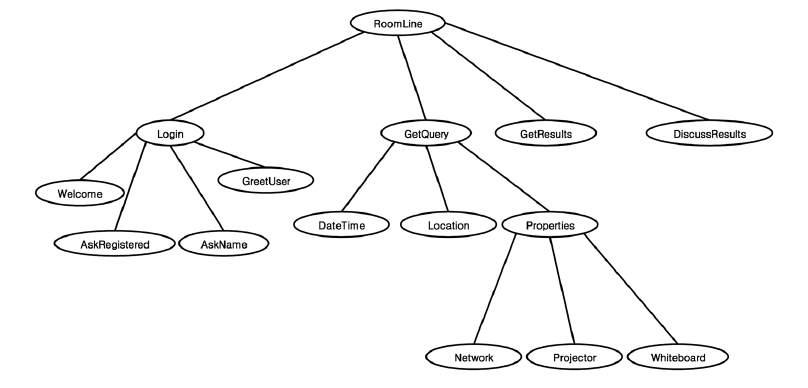
\includegraphics[width=12cm]{figures/knowledgeDM.png}
\caption{基于RavenClaw框架的RoomLine对话管理策略树}
\label{fig:knowledgeDM}
\end{figure}


\item 数据驱动的对话管理

最近几年,对话管理的研究趋势逐步转向数据驱动的方法,即通过语料库来训练相关对话结构和知识库。虽然这种数据驱动的方法需要消耗很大的时间和人力进行语料库标注,但是对话管理模型的训练几乎不需人工干涉,而且在可移植性方面,如果需要在其他领域建立一个对话系统,也只需要重新训练新的语料库,与基于知识的对话管理相比,这显然是更简便的方法。

这些优势驱动了使用无监督强化学习的随机对话建模的发展,如\cite{Levin2000}使用了基于马尔可夫决策过程(MDP)的强化学习算法,\cite{WilliamsYoung2007, Young2013, Williams2013, Kim2015, Henderson2013}使用了基于部分可观测马尔可夫决策过程(POMDP)的强化学习算法来进行对话建模。这些对话管理框架都使用数据驱动的统计机器学习算法,通过强化学习算法来优化系统的奖励或者惩罚函数,允许系统有理论原则性地根据当前的对话状态来动态修改对话策略。此外,基于POMDP的对话管理还能通过支持最优语音识别和自然语言理解结果来评估信念状态(belief state),从而达到纠正语音识别以及自然语言理解模块中出现的错误。对于基于POMDP的对话管理,系统只观测在当前状态下的有关现实世界(在对话系统中指的是语音识别和自然语言理解结果)的不完整的信息,系统必须利用当前对话状态下寻求一种最优策略将当前的信念状态映射到对话管理策略上。因此,基于POMDP的对话管理可以通过维持信念状态(即最优语音识别和自然语言理解结果)分布来实现语音识别和自然语言理解结果的纠错处理,而无需其他特殊方法。同时,有关用户的背景知识(如用户的特长以及情感状态等)也能通过可分解的强化学习模型映射到状态空间中,从而使得对话管理更人性化。

尽管强化学习算法在理论上能解决基于不确定性的推理和决策,从而为对话管理提供了有效的途径,但在实现过程中,基于强化学习的对话系统依然困难重重\cite{Paek2006},首先,对话系统中的状态包含大量语义项和项值、用户意图、理解结果和对话历史的各种可能组合,使得状态空间的规模指数增长\cite{Yukai2014},因此使得强化学习的过程计算复杂度巨大,也使得对话控制的精细改进过程变得困难;其次,强化学习得到的最优策略也剥夺了对话系统开发者对对话流程的监督指导权利。\cite{WilliamsYoung2005, Lemon2006, Young2007, Thomson2008, Williams2008b}在一定程度上对这些问题进行了改进。\cite{Lemon2006, Williams2008b}中研究了如何将传统的基于知识的对话管理和基于强化学习的对话管理结合起来构建商务领域的对话管理规则库,在一定程度上给开发人员留下了对对话管理的监督和指导的空间。然而,目前该方法仍在研究中,尚未用到实用性的对话系统中。

数据驱动的对话管理方法还包括使用最大似然估计等有监督的机器学习算法从对话语料库中训练对话模型\cite{Hurtado2005}。为了避免数据稀疏的问题,\cite{Hurtado2005}中采用了对话寄存器来表示对话状态序列用于跟踪对话历史,其中对话寄存器包含用户在整个对话历史中提供的各项信息。

基于实例的对话管理方法也是数据驱动的对话管理中的一个流行的研究方向,具有代表性的系统有\cite{Murao2003, Inui2001, Lee2009c}。该方法假定类似的对话状态会引发类似的回应,因此可以通过匹配对话实例库中的与当前对话状态最相似的对话状态来构建相应的对话模型。目前搜索与当前对话状态最相似的对话实例大多数都使用关键词来检索,对话实例库中的对话实例的表示通常采用语义约束的形式,从而整个对话实例库可以通过语义索引来概括\cite{Lee2009c}。对话管理模块首先将当前的对话状态也表示为语义约束的形式,并试图从对话实例库中找到与之相近的对话实例,如果没有返回结果,系统会放松语义约束后再一次从对话实例库中查找相近的对话实例;如果返回结果不止一个,那么系统会采用启发式算法来计算返回结果中的每一个实例与当前输入的相似度,然后选择相似度最高的返回作为应答。

数据驱动的对话管理的相关研究在近几年来发展可以说是突飞猛进,当下流行的深度机器学习也被用于对话管理领域,通过深度神经网络在大型对话语料库上训练对话模型的研究也取得了比较有前景的实验结果\cite{Shang2015, Sordoni2015b, VinyalsLe2015}。近期的相关研究还包括“端到端”的数据驱动对话管理框架,也就是利用多层次的神经网络对整个对话过程中的每一个组件以及每一个阶段都进行训练,从而得到包含从语音输入到语音输出,以及对话过程中各个阶段的一系列概率模型\cite{Serban2015}。然而,这些数据驱动的方法都严重依赖于足够大的数据集,为了取得有价值的实验结果,动辄需要上千万甚至上亿则对话。

\item 基于混合方法的对话管理

为了克服上述提到的基于知识以及数据驱动的对话管理方法中的各种不足,基于混合方法的对话管理的研究逐渐发展起来。

传统的基于强化学习的对话管理方法需要通过用户和系统的反复交互来学习一个好的对话策略,而且目前的强化学习算法的泛化能力很弱,往往需要通过大量人力去和系统交互或者庞大规模的对话语料库去归纳一个很小语境条件下的对话策略。为了解决该问题,\cite{Pietquin2006, Schatzmann2007} 中引入了用户模拟器的技术,也就是说,通过用户模拟器来代替人和对话管理器进行交互。根据有限的真实语料概括学习得到特定的用户模型,用户模拟器可产生大量的模拟对话。除此之外,\cite{Henderson2008}中还提出了将强化学习和有监督学习结合起来并在有限固定的对话语料库上学习和优化对话策略的混合方法,有监督学习的引入在一定程度降低了传统强化学习方法中对巨大对话语料库的需求程度。在该方法中,强化学习用于优化对话策略中对话奖惩的度量,而有监督学习用于指导对学习到的对话策略状态空间的剪枝,从而得到更高效有用的状态空间。

在传统的POMDP算法中,优化过程可以在任何时刻选择任意的行为,因此,没有简洁易操作的方式引入一些领域相关的常识性知识来约束和指导优化过程。例如,一个医疗相关的对话系统不应该在问病人症状之前就提供用药建议,然而,传统的POMDP算法却不存在直接的方法将该常识引入到优化过程中。近年来,也有相关研究提出来改进该问题,如\cite{Lemon2006, Williams2008b}中提出了在POMDP框架中基于传统规则来约束策略状态中的可能对话行为的集合,这样通过传统规则来对状态空间中的一些不合理的行为进行剪枝,不但加速了强化学习的优化过程,也使优化过程往更可靠的方向进行。

目前,传统的基于实例的对话管理方法应用在实用口语对话系统中还存在很多关键问题,比如先验知识的缺乏,语音识别的错误,以及语义解析的不确定性等。针对这些问题,\cite{Lee2009b}中提出了将对话实例与先验知识同时用在基于实例的对话管理中,从而提高系统的鲁棒性。该方法使用了基于议程的模型,将先验知识表示为议程图,并作为对话管理的子任务流之一来对领域相关的对话控制进行编码。这些先验知识不仅被用于预测系统的下一个对话行为,还通过议程图来跟踪对话状态,以便于处理一些话题焦点转移的意外情况。另外,该方法还通过在话语层次和语篇层次上的打分作为启发,来对当前对话状态下的N-best的对话行为假设进行重排。

基于混合方法的对话管理的最新研究趋势还包括在强化学习模型中引入概率规则的概念,\cite{Lison2015}中将概率规则定义为逻辑条件和概率事件之间的结构映射,并作为高层次的模板用于概率图模型中,其中可能包含未知参数,其值可以通过数据进行贝叶斯推断来估计得出。由于使用了逻辑的抽象化,这些概率规则可以对数据驱动的基于POMDP的对话管理中使用的概率模型进行编码成更紧凑更可读的形式。在理想情况下他们需要较少的参数估计,因此,与典型的基于POMDP的对话管理方法相比,要求较少的训练数据,也允许开发者在对话管理过程中使用人工编写的对话控制规则。然而,该方法还未成熟和完善,其实用价值在很大程度上还有待考察。

\end{enumerate}

在这些繁多的对话管理研究技术中,本文提出的方法更接近于现有技术中的通用对话建模技术,以及最新的在对话管理中引入概率规则的相关研究。然而,与这些研究又不同,本文由系统的动机出发,结合言语行为以及其他的交际行为与这些动机之间的关系来构建一个相当复杂的对话管理模型。此外,由于使用了基于概率逻辑规则的知识表示方法,本文的认知对话管理框架也能通过观测数据来进行对话模式的自适应。因此,本文的方法可以被认为是基于混合方法的对话管理。
从长远角度来看,本文提出的对话管理框架将实现以通过观测数据来进行经验概率分析为主的对话控制,不过目前,我们的研究集中于将其内置的通用对话建模将作为对话行为控制的主导。


%%%%%%%%%%%%%%%%%%%%%%%%%%%%%%%%%%%%%%%%%%%%%%%%%%%%%%%%%%%%%%%
\subsection{自然语言理解、生成研究综述}{Overview of Natural Language Understanding and Generation}
%%%%%%%%%%%%%%%%%%%%%%%%%%%%%%%%%%%%%%%%%%%%%%%%%%%%%%%%%%%%%%%

智能对话系统的研究、开发和使用都离不开自然语言理解和自然语言生成的支持,因此本小节将分别对自然语言理解和自然语言生成方面的现有研究技术以及存在的问题等进行简要的回顾。

\begin{enumerate}

\item{自然语言理解}

自然语言理解是自然语言处理(NLP)的分支领域,它是通过使用软件来理解自然语言的意义(语音,或者本文更关注的“文本”)。自然语言理解主要是将自然语言转换成抽象的语义形式,以获取语言的含义;或者是转换为某种响应(例如对某个问题的回答),以说明其理解了语言的含义。

在20世纪80年代之前,自然语言理解的方法通常是基于人工编写的复杂规则。紧随着机器学习技术的发展,基于统计的自然语言理解方法也开始兴起\cite{Tan1992}。乔姆斯基的形式语法理论以及摩尔定律使得通过语料库来进行统计学习的自然语言理解技术成为可能\cite{Gupta2014}。近些年来,越来越多的相关研究投入到无监督学习或者半监督学习方法上,这些技术能使自然语言理解不那么依靠需要大量人力获得的人工标注的语料库。一般来说,与有监督学习相比,无监督学习或者半监督学习的难度相当大\cite{Gupta2014}。

在目前主流的智能对话系统中,自然语言理解模块通常通过以下流程逐步完成:词法分析、句法分析、语义关系抽取、语义理解。词法分析主要是将字符序列转换为标记序列的过程,并非本文的研究内容,因此这里从其他几方面来介绍各流程的研究现状。


\begin{description}
\item[(1)]{句法分析}
通常自然语言理解是通过对句子的某些,或全部句法法进行分析来完成的。大量的形式化体系和算法通过特定的语法体系对句子的句法结构进行解析。大体来说,主流的句法分析包括“依存句法分析” \cite{Eisner1996a, Eisner1996b, Yamada2003} 以及 “短语结构句法分析” \cite{Chomsky1957, Pollard1994}。短语结构句法分析依据短语结构文法\cite{Thompson1981, Charniak1997, Makino1998, Charniak2006},首先对句子进行短语分析,然后指出单词和短语之间的关系,以及短语之间的关系;而依存句法分析依据依存文法\cite{Tesniere1959, Melchunk1988},仅仅在句子中的单词之间标注(有标记的)连接关系。依存句法分析是我们要在本文中探讨的语法类型。


这里的“依存”是指语言单位(如单词)由有向链接相互联系在一起。一般来说,在依存语法中,(限定)动词被视为句子或子句结构的中心,其它所有句法单位(单词)是直接或间接地与动词通过有向链接相连。这种有向链接被称为“依存”。句子结构是由一个词(中心词)与它的依存词之间的关系而决定的。


“依存”关系是一对一的对应关系:对于句子中的每个元素(例如:单词或语素)来说,实际上句子中都有一个与其相对应的节点。这种一对一的对应关系决定了“依存语法”就是单词(或语素)的语法。所有的句子都有元素和将元素组成结构的依存关系,这种情况应该与短语结构语法的“成分关系”进行比较,“成分关系”是一对一,或一对多的对应关系,也就是说,对于句子中的每个元素来说,有一个或多个与其对应的节点。这种不同带来的结果是:相比短语结构,依存结构非常紧凑,因为它往往包含很多小的节点。从计算机处理的角度来说,这种简洁的结构是有益的。


\item[(2)]{关系抽取}
自然语言理解中的一个重要方向是{\bf 关系抽取}。在NLP领域中,关系抽取已成为一个重要的研究方向,一方面是因为它的实际应用价值,另一方面因为它被看做是语义分析的一部分,而且是目前的技术相对容易实现的那部分。到目前为止,吸引最多注意力的关系抽取是命名实体之间的关系识别,例如:“个人从属关系”和“组织地址关系”。

一般来说,关系可以由一个元组的形式来定义的,$t = (e_1, e_2, ...,e_n)$。在这里,$e_i$ 是文本中预定义关系$r$ 的实体。大多数关系抽取系统主要关注二元关系的抽取。例如 :

\begin{verbatim}
位于(厦门,中国)
father-of(Richard Li, Li Ka-Shing)
\end{verbatim}

抽取“高阶关系”也非常有意义。例如这个句子:"At codons 12, the occurence of point mutations from G to T were observed'' (“在密码子12,观察到从G到T的点突变”)。句子中出现了一个4进制生物医学关系,可以描述为:

\begin{verbatim}
point mutation(codon, 12, G, T)
\end{verbatim}

目前人们普遍视“关系抽取”为一个有监督分类问题,它从一个语料库开始(语料库中包含由人类标记的相关语义关系),然后利用统计方法来对标记的关系建模,并学习出适合应用于其它文本的统计模型。

目前,关系抽取系统的主要限制在句子层面上运用。事实上,关系可能跨越句子,甚至贯穿不同的文件。然而,解决这一问题需要一定的常识和非常灵活的知识表示。本文的研究也无法直接解决这一问题,但我们相信:通过将句子意义映射为通用的知识表示,我们已经奠定了解决问题的基础。在这种知识表示中,跨句或跨文本的通用联系和推理是可以被实现的。

\item[(3)]{流结构语法}


将流结构语法(FCG)与本文使用的语言形式化体系进行比较分析是很有意义的。在FCG中,一句话语的信息是以语义和句法结构组织在一起的。语义结构是对“话语意思”的分解,它含有特定语言的语义分类,例如:“put”事项被归类为“起因-移动-位置”类事项,包括一个施事者(agent)、一个受事者(patient)和一个位置(location)。句法结构是将话语形式分解为成分和词素,还包含附加的句法分类,比如:句法特征(例如:数量和性别)、词序限制等。


从理论上来说,FCG是基于一种程序性语义的方法,在这个意义上,话语的意思是听话人假定要执行的程序,因此,概念化便是一个规划过程(规划该程序),而解析便是对该程序的执行过程。
FCG中,有关配对句法和语义结构的例子(短语“the ball”),请见图 \ref{fig:fcg1} and \ref{fig:fcg2}。

\begin{figure}[htb]
\centering
\includegraphics[width=12cm]{figures/fcg1.png}
\caption{ FCG中对短语“the ball”的句法及语义表示结构}
\label{fig:fcg1}
\end{figure}

\begin{figure}[htb]
\centering
\includegraphics[width=12cm]{figures/fcg2.png}
\caption{ FCG中对短语“the ball”的语义表示的列表形式}
\label{fig:fcg2}
\end{figure}


所有的FCG规则都是双向的。通常在产生过程中,所要表达的语义内容是与语义结构相统一的,有可能产生一组绑定。如果成功了,绑定会与语义结构相融合。这种融合可以理解为“部分统一”,但它利用结构中那些遗漏部分扩展了结构。在句法分析过程中,被分析的句子与句法结构是统一的,同时,结果中的某些部分被添加到语义结构中。
\end{description}

本文所使用的形式化体系在概念上有些类似FCG。 此外,我们有配对句法和语义结构,而且还进行双向处理。在第\ref{chap:comprehension}章中,我们将论述链语法,它将句子转换成句法结构,以及RelEx和RelEx2Logic模块,它们将句法结构转换成语义结构。在第 \ref{chap:generation}章中,我们将阐述另一个方向的Microplanner 和SuReal模块,也就是将语义结构转换成句法结构,再生成句子。本文研究的平台OpenCog中的模式匹配器(Pattern Matcher)在使用这些句法和语义结构时,也将这些结构视为有效的程序,同样实现了“程序化语义”。但我们的形式化体系与FCG的着重点不同。FCG主要是用作探索问题的理论工具,而本文的研究更侧重用于真实世界的实际应用。

\item{自然语言生成}{Natural Language Generation}

随着统计机器学习技术不断成熟和发展以及大数据的利用率不断提高,统计的方法已经被广泛用于自然语言理解的很多模块,如句法分析、语义关系抽取,甚至对话系统中的对话管理模块,并取得了很大的进展;然而,由于语义标注语料的缺乏,数据驱动的自然语言生成技术还面临着诸多困难和挑战,目前大部分自然语言生成系统仍然采用了基于规则的方法\cite{Cheyer2007, Mirkovic2011}。

自然语言生成(NLG)是自然语言理解(NLU)的反向过程。总的来说,自然语言生成是从信息的计算表示中自动生成人类(自然的)语言。由于语义知识表示体系的差异化,造成自然语言生成系统的输入多样化,因此不同的自然语言生成系统所包含的组块一般都不尽相同。概括地说,自然语言生成系统可以表示为解决下列两项任务:

\begin{itemize}
\item What should I say?(我应该说什么?)
\item How should I say it?(我应该怎么说?)
\end{itemize}

为了解决这些问题,自然语言生成系统可能涉及许多相互关联的规划模块,如:
\begin{itemize}
\item 确定要表达的信息
\item 构建语篇规划
\item 将信息块转换为语篇单位
\item 选择适当的短语和单词
\item 输出正确的语法
\end{itemize}

将这个流程分解为阶段的方法如下:
\begin{description}

\item [1)] 宏观规划

宏观规划涉及选择和组织内容。它输入的是一个或多个沟通目标:解释、描述,或提问;引起听众的某种行动或思考等。宏观规划输出的是一种知识架构,这个架构不一定是语言的属性,而是体现智能体所要沟通的信息。除了一般性内容,这种知识架构可能包含一些与沟通过程有关的信息,例如:不同的知识块应该以什么样的顺序来传达。

目前宏观规划的研究主要基于一些语篇结构层次上特定的理论体系,例如:修辞结构理论\cite{Mann1987}。在本文所介绍的研究中,我们采用了基于动机认知模型Psi的宏观规划,该模型的构建非常符合人类的心理特征。

\item [2)] 微观规划

微观规划则运用知识架构,并将它们分为句块。微观规划必须处理多种语言问题,例如:

\begin{itemize}
\item 句子范围:是否可以将两片叶子接在一起,怎样接在一起。(“我今天饿了。我去了 Burger King。” VS “我今天饿了,所以我去了Burger King。”)
\item 代词化
\item 聚合:删除重复内容。(“抽烟对你不好。抽烟会缩短你的寿命。抽烟让你口气不佳” VS “抽烟对你不好、缩短你的寿命,而且让你口气不佳”)
\item 主题化
\item 主题排序
\end{itemize}

到目前为止,大多数微观规划都是为特定的应用而专门制定的。比较典型的多用途微观规划框架如SPUD\cite{Stone1997},它利用的是一个基于逻辑的规划流程形式。尽管在细节上有所不同(原来的SPUD是基于树-邻近语法),但我们所描述的微观规划在概念上受到了SPUD的很大影响。

\item [3)] 表层生成

最后,“表面生成”涉及的是文本表层的生成,例如:把知识结构转换为句子。经典的表层生成器,例如FUF/SURGE\cite{Elhadad1992}和 Penman/KPML\cite{Matthiessen1991},都是以深层语言学理论为基础的。其他知名的系统,例如Nitrogen\cite{Langkilde1998}则采用的是统计法。所有基于规则的方法和统计法现在仍然流行。

\end{description}

\end{enumerate}

在对话系统方面的应用方面,自然语言生成的主要任务是将对话管理生成的抽象对话行为组块转换成恰当的应景的自然语言文本,通常,这里的抽象对话行为组块包含对话行为类型以及相应的(属性,值)二元组,如图\ref{fig:NLG-example-litReview}所示\cite{Wen2015}。有关这方面的研究,早期的方法有使用N-gram语言模型来对一些人工编写的语言生成器产生的可能输出结果进行重排\cite{Langkilde1998},显然该方法需要依靠大量人力来编写规则来构建语言生成器。为了减少人工编写的语言生成器的使用,\cite{Oh2000}使用基于N-gram的语言模型生成器组合来替代了这些人工编写的语言生成器,针对每一个对话类型定义一个相应的N-gram生成器,虽然\cite{Oh2000}中将人工编写的规则的使用限制在后处理的小集合上,但还是无法避免生成器产生冗余不必要的短语和句子的情况,从而使计算复杂度相当大,而且N-gram的方法也无法判断输出的结果就是包含对话行为组块中最多相关语义项的句子或文本。\cite{Mairesse2010, Mairesse2014}中提出了基于统计的以短语为生成单位的自然语言生成方法,该方法使用了统计方法在带标注的话语语料库中训练出(话语,粗糙语义概念)的二元组,从而根据抽象对话行为组块的属性值得到相关的短语或句子。该统计方法在一定程度了解决了需要大量人力来编写规则的难题,但是带语义概念标注的语料库并不成熟也很难收集,而且统计方法相对耗时,因此使得该方法很难扩展到新的领域。

\begin{figure}[htb]
\centering
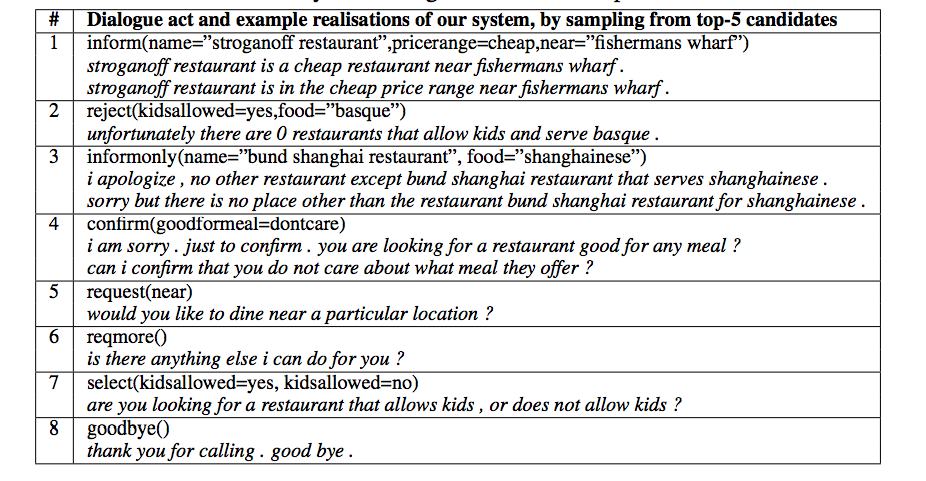
\includegraphics[width=12cm]{figures/NLG-example-litReview.png}
\caption{对话系统中自然语言生成模块的抽象对话行为实例}
\label{fig:NLG-example-litReview}
\end{figure}

针对上述这些问题,\cite{Wen2015}将深度学习的方法应用到自然语言生成领域,使用递归神经网络(RNN)和卷积神经网络(CNN)的结合来训练对话行为类型和话语的二元组。该方法无需任何的语义对齐二元组或者预先定义的语法树等标注语料库的指导,因此可以在任何领域的对话语料库上进行模型训练,使其扩展性得到了很大的提高,与上述提到的系统相比,该方法得到的实验结果也有明显的改善。但该方法只是训练出对话行为类型和话语的配对,无法用于针对抽象的语义表示形式的语言生成,然后一个好的智能对话系统中,要求的对话往往需要通过语义分析和一定的逻辑推理来生成。

总的来说,与自然语言理解相比,自然语言生成技术要落后得多。目前的实用系统往往限定在一些专业领域,而且很粗糙。概念比较先进的系统,如FCG,尚未经过广泛地实践测试。正如第\ref{chap:generation}章中所介绍的,我们在这一领域的研究代表了“基于规则的方法”和“统计法”的融合。我们认为这种融合非常有前景,但目前还没有精细化,也没有经过系统性评估。

%%%%%%%%%%%%%%%%%%%%%%%%%%%%%%%%%%%%%%%%%%%%%%%%%%%%%%%%%%%%%%%
\subsection{言语行为理论及相关研究综述}{Overview of Speech Act Theory and related research}
\label{sec:speechAct}
%%%%%%%%%%%%%%%%%%%%%%%%%%%%%%%%%%%%%%%%%%%%%%%%%%%%%%%%%%%%%%%

我们认为,分析和管理对话系统需要产生的各类话语的一个有效方法是:使用由Austin\cite{Austin2005}提出,Searle\cite{Searle1969} 改进的言语行为理论(Speech Act Theory)。本文将要阐述的智能对话研究中正采用了此方法,且在研究过程中,我们发现这个理论是极其有用且方便使用的。我们在这一节先回顾言语行为理论的基本观点,并介绍一些言语行为理论在对话方面的相关研究以及更细致具体的分类体系。

言语行为理论是语言学和语用学等研究中的一个重要理论。言语行为理论的核心概念是:强调语言的意向功能,认为说话者在说话的同时是在实施某种行为。因此,根据言语行为的观点,分析说话者的语言行为的过程,也就是说话者分析为了实现某个特定目标而采用的一系列的言语行为的过程。

言语行为理论探讨那些可以通过言语来表现的行为类型。Austin\cite{Austin2005}将言语行为分为以下几种:

\begin{itemize}
\item {\bf 言内行为(Locutionary Act)}:话语的外在表现形式,即:话语本身的字面意义。
\item {\bf 言外行为(Illocutionary Act)}:话语的“言外之力”,即:说话者对受话者的影响。
\item {\bf 言后行为(Perlocutionary Act)}:话语达到的实际效果,即:话语所导致的行为,如说服、劝说、吓唬、启发、激励,或者让受话者去做某件事,或者让受话者意识到什么,不论是有意还是无意的。
\end{itemize}

Searle对Austin提出的言语行为理论做了深入的研究和探讨。在Searle\cite{Searle1969}看来,言语行为有时仅仅指的是言外行为。他认为,说话人通过他们的言语只能获得5类言外之力,它们分别是:

\begin{itemize}
\item 断言类:说话人自己承诺事情是真的。The sky is blue. (天是蓝色的。)
\item 指令类:说话人试图让受话人做某事。Clean your room! (打扫你的房间!)
\item 承诺类:说话人对未来的行为做出承诺。I will do it. (我将会做这件事。)
\item 表达类:说话者表达了某些心理状态。I’m Sorry. (对不起。)。
\item 声明类:说话人带来了不同的状况。The meeting is adjourned.(这个会议休会了。)
\end{itemize}

受这个本体论的启发,Twitchell 和 Nunamake在他们2004年的论文(标题为:言语行为归档:分析持续谈话和其参与者的概率统计法。\cite{Twitchell2004})中提出了更加精细的“42种言语行为”本体论,叫做SWBD-DAMSL (DAMSL = Dialogue Act Markup in Several Layers)。尽管有少量不符合Searle的观点,并被分类为“其它”,但几乎他们所有的42种言语行为类型都能够被映射到Searle的5个高级类别之一。图\ref{fig:DAMSL}和\ref{fig:Searle}描述了这42种行为和它们与Searle分类之间的关系。我们已经利用了这个Searle解析法,它给我们正在进行的自然语言对话研究带来了灵感。

\begin{figure}[htb]
\centering
\includegraphics[width=12cm]{figures/DAMSL.png}
\caption{SWBD-DAMSL中使用的42种言语行为}
\label{fig:DAMSL}
\end{figure}

\begin{figure}[htb]
\centering
\includegraphics[width=12cm]{figures/Searle.png}
\caption{ 42种SWBD-DAMSL言语行为类型与Searle的言语行为类型的关联}
\label{fig:Searle}
\end{figure}


总之,言语行为理论为对话管理和对话控制提供了一个新的思路,也就是将对话的话语看成是一种行为,这样不仅能通过对不同言语行为的定义来猜测说话人的意图,还能将对话行为看成和其他非语言的行为类似。不难看出,它不仅给对话管理和对话控制提供更多可行的用于非语言的行为控制机制,也同时能将对话与智能体的其他行为有效结合起来,从而完成更智能更人性化的对话。

%%%%%%%%%%%%%%%%%%%%%%%%%%%%%%%%%%%%%%%%%%%%%%%%%%%%%%%%%%%%%%%
\section{存在的问题}{Omissions of Present Research}
%%%%%%%%%%%%%%%%%%%%%%%%%%%%%%%%%%%%%%%%%%%%%%%%%%%%%%%%%%%%%%%

XXXXXX需要修改:按照上面的顺序来介绍每一领域的相关研究出现的问题,即知识表示逻辑推理、言语行为理论的应用、对话系统、自然语言理解和生成。

虽然上述工作已经取得了重要成果,但是从一个更广阔的视野来看,仍然还有很多未完成的工作,其中有许多也是我们目前正在研究和开发的课题。

首先必须强调的是,截止到我们目前所做工作为止,语言理解和生成的许多关键方面一直未被关注,甚至完全被忽略。如以下几个例子:
\begin{itemize}
\item 形态。链语法分析器,作为上述理解系统的初始阶段,最近已扩展到在语素及文字水平进行句法分析;但我们还没有将这项工作纳入到我们自己的工作中。
\item 语用。我们能够按照他们的实际能力对语句生成逻辑表达式进行分析,但是我们并未执行语用方面的分析。
\item 消歧。我们已在OpenCog框架中实现了一个简单词义消歧系统,但还没有集成到本文的工作中。
\item 名词的回指消解。在我们的理解系统内,人称代词的指代消解已通过各种启发式算法实现,但名词的回指却被忽略。
\end{itemize}

目前我们工作的一部分是指出整体框架中的这些缺陷。然而,我们相信即使给出这些疏漏,我们所做的工作也足够为以上三个假设提供合理的证据支持。展示处理上述现象能力必然有助于compelling system,但是对于验证本方法和三个假设的有效性并不必要。

本文工作的其中一个目标就是构建一个具有一定智力水平的智能会话系统。为了实现这样的智能会话系统,本文也开发了涉及自然语言理解、生成和推理等的相关模块。但本文的工作并不仅仅包括自然语言理解、生成和推理本身,例如还包括下面几个方面:
\begin{itemize}
\item 来自语言的逻辑表达和来自其他信息渠道的逻辑表达的有效整合,这些其他信息渠道可以是机器人或虚拟世界里的涉身知识,也可以是限定领域的标注语料库
\item “对话控制程序”的实现,该对话控制程序从一个动机驱动的系统中获取相关信号,然后结合系统当前的动机、最近的语言输入以及当前的系统知识等相关语境知识来选择相应的语言应答。
\item 额外的推理控制机制,使得智能体在被不相关或者不完全相关的信息来源打断后,仍能进行相对复杂的推理,从而给出相关的应答。
\end{itemize}

这些模块将在第 \ref{chap:dialogueModel}和\ref{chap:dialogue}章介绍。这些工作目前还无法在所有的语言现象中得到了验证,还有待进一步深入研究。然而, 在理解、生成和推理等方面,明确的研究方向和相关工具的实现,无疑为以后的研究奠定了结实的基础和提供了一个便捷的研究平台。我们提出三个核心假设的主要原因,是因为它们提供了一种有效的方法,能够借助自然语言理解、生成和语义推理等子系统,来搭建一个大型的智能对话体系结构。

%%%%%%%%%%%%%%%%%%%%%%%%%%%%%%%%%%%%%%%%%%%%%%%%%%%%%%%%%%%%%%%
\section{研究目标和内容}{Goals and Contributions}
%%%%%%%%%%%%%%%%%%%%%%%%%%%%%%%%%%%%%%%%%%%%%%%%%%%%%%%%%%%%%%%
提出创新点

%%%%%%%%%%%%%%%%%%%%%%%%%%%%%%%%%%%%%%%%%%%%%%%%%%%%%%%%%%%%%%%
\section{论文的组织结构}{Outline}
%%%%%%%%%%%%%%%%%%%%%%%%%%%%%%%%%%%%%%%%%%%%%%%%%%%%%%%%%%%%%%%


